%% This document gives an example on how to use the ntnumasterthesis
%% LaTeX document class.

%% Use short name MACS, MIS, CIMET, MTDMT, MIXD or MIS  
%% Language english or norsk
%% b5paper with oneside or twoside, you can set A4 if you want but you submit in b5

%% If you want print with the heading material on a4 paper you can use this format
%% \documentclass[MACS,english,a4paper,oneside,12pt]{ntnuthesis/ntnuthesis}

%% with the change to using DAIM we have a new option. include DAIM after english below removes the front page material so that you can then submit in the DAIM system. If you are wanting the front material remove DAIM and make sure you fill in the DaimData.tex file.
\documentclass[MIS,english]{ntnuthesis/ntnuthesis}

\usepackage[T1]{fontenc}
\usepackage[utf8]{inputenc}     % For utf8 encoded .tex files allows norwegian characters in the files. This can be dangerous if you change to a differnt editor.
%\usepackage[pdftex]{graphicx, hyperref}   % For cross references in pdf
\usepackage{graphicx}
\usepackage{hyperref}   % For cross references in pdf

\usepackage{pgfplots}
\pgfplotsset{width=\hsize,compat=1.15}

% For smart references 
%    use \cref{label} and Caption and Number will be added automatically
\usepackage[capitalise,noabbrev]{cleveref} 

\usepackage{color}              % For colouring text 
\hypersetup{colorlinks=true,     
		linkcolor=blue,          % color of internal links (change box color with linkbordercolor)
    citecolor=blue,        % color of links to bibliography
    filecolor=blue,      % color of file links
    urlcolor=blue           % color of external links
		}
\usepackage{csvsimple}  % for simple table reading and display
\usepackage{url}
\usepackage{booktabs}
\usepackage{gnuplottex} %miktex option if using miktex on windows
\usepackage{rotating}


\definecolor{darkgreen}{rgb}{0,0.5,0}
\definecolor{darkred}{rgb}{0.5,0.0,0}

\lstset{        basicstyle=\ttfamily,
                keywordstyle=\color{blue}\ttfamily,
                stringstyle=\color{darkred}\ttfamily,
                commentstyle=\color{darkgreen}\ttfamily,
}

%Typesetting of C++ but not always stable in titles etc...
\newcommand{\CPP}[0]{{C\nolinebreak[4]\hspace{-.1em}\raisebox{.1ex}{\small\bf +\hspace{-.1em}+\ }}}

%\usepackage[table]{xcolor}% http://ctan.org/pkg/xcolor
%\usepackage[nomessages]{fp}
%\newlength{\maxbarlen}


\newcommand\databar[3][gray!20]{%
  \FPeval\result{round(#3/#2:4)}%
  \rlap{\textcolor{#1}{\hspace*{\dimexpr-\tabcolsep+.5\arrayrulewidth}%
        \rule[-.05\ht\strutbox]{\result\maxbarlen}{.95\ht\strutbox}}}%
  \makebox[\dimexpr\maxbarlen-2\tabcolsep+\arrayrulewidth][r]{#3}}



\newcommand{\com}[1]{{\color{red}#1}} % supervisor comment
%\renewcommand{\com}[1]{} %remove starting % to remove supervisor comments
% This will appear in text \com{Lecuters comment} and be visible unless you uncomment
% the renewcommand line.

\newcommand{\todo}[1]{{\color{green}#1}} % items to do
%\renewcommand{\todo}[1]{} %remove starting % to remove items to do

\newcommand{\n}[1]{{\color{blue}#1}} % other comment
%\renewcommand{\n}[1]{} %remove starting % to remove notes

\newcommand{\dn}[1]{} % add the d to a note to say that you have finished with it.





% Set to true ONLY if using Harvard citation style
\newboolean{HarvardCitations}
\setboolean{HarvardCitations}{false} % false for computer science, true for interaction design and harvard style


\ifthenelse{\boolean{HarvardCitations}}{%
	\usepackage{natbib} % for Harvard names as citations.
}{%
	\usepackage[numbers]{natbib} % for Vancover numbers in bibliography
}

\newcommand{\q}[1]{\leavevmode\marginpar{\small\em #1}}
\renewcommand{\q}[1]{}


\begin{document}

% for students submitting in the DAIM system this information will not be used.
% their is an option for DAIM submission which removes this information and checks it is B5.
% Removing the DAIM option on the document type will use this material.

\setthesistitle{Real Time Windows Event Log Analysis}
\setthesisshorttitle{Real Time Windows Event Log Analysis} % a short version for the page headers if your normal title is too long to fit
\setthesisauthor{Martin Ingesen}
\setthesissupervisor{Prof. ?}
\setthesissupervisorA{Prof. ?}  % if you have a second supervisor add it like this
%\setthesissupervisorB{Prof. Smart Guy}  % if you have a second supervisor add it like this


\nmtkeywords{Thesis, Latex, Template, IMT}
%\nmtdesc{This is the short description of a masters thesis}


\setthesisdate{12-12-2019}
\setthesisyear{2019}



%for CIMET theses you need to see all of these as well

%\setthesiscampus{Gj\o{}vik}
%\setthesisHostInstitution{\NTNU}
%\setthesisHostInstitution{University of Eastern Finland}
%\setthesisHostInstitution{Universit\'e Jean Monnet Saint-Etienne}

%\setthesisjuryA{} %jury names
%\setthesisjuryB{} %jury names
%\setthesisjuryC{} %jury names
%\setthesisjuryD{} %jury names


 % this is the file which contains all the details about your thesis
\makefrontpages % make the frontpages
%this is the intro to the thesis
\include{inc/preface}

\include{inc/acknowledgments}

\include{inc/abstract}


\tableofcontents

\hypersetup{pageanchor=true}

% Comment with a percent to remove figures or tables:
\listoffigures
\listoftables
\lstlistoflistings

\chapter{Definitions/Terms}
\label{chap:definitions}

\subsubsection{Context} -
\subsubsection{Context Engine} The part of the program that handles context.
\subsubsection{Event} A single Windows Event Log event.
\subsubsection{Goroutine} A lightweight thread handled by the Go runtime.
\subsubsection{Log line} A single line of a dataset, which consist of a single event.
\subsubsection{Sysmon} A Windows service and driver that uses XML configuration files to enhance the log data given by Windows Event Log.
\subsubsection{Windows Event Log} A built-in mechanism in Windows that logs telemetry of what happens on the system. Can be enhanced by installing and configuring Sysmon on the system.
\subsubsection{Worker} -

\chapter{Datasets}
\label{chap:datasets}

\section{Evaluation of existing datasets?}

\subsection{Boss of the SOC}
\todo{Describe the BOTS-datasets}
\todo{Run some actual tests against the dataset to see if we get a hit with our rules}

\subsubsection{Version 1}
\url{https://github.com/splunk/botsv1}
\subsubsection{Version 2}
\url{https://github.com/splunk/botsv2}
\subsubsection{Version 3}
\url{https://github.com/splunk/botsv3}

\subsection{Mordor}
\url{https://github.com/hunters-forge/mordor}

\subsection{EVTX-ATTACK-SAMPLES}
\url{https://github.com/sbousseaden/EVTX-ATTACK-SAMPLES/}



\section{Mordor datasets}
The Mordor datasets are pre-recorded events generated by simulating adversarial techniques in a test environment using common red team tools like Empire and Cobalt Strike. The largest dataset in the collection aims to simulate a Advanced Persistent Threat (APT) known as APT3/Gothic Panda. The dataset contains two scenarios, both outlined in MITRE ATT\&CK Evaluation Operational Flow. The flow maps directly to MITREs ATT\&CK framework, by stepping through 10 different "steps".

\begin{enumerate}
\item Initial Compromise
\item Initial Discovery
\item Privilege Escalation
\item Discovery for Lateral Movement
\item Credential Access
\item Lateral Movement
\item Persistence
\item Collection
\item Exfiltration
\item Execution of Persistence
\end{enumerate}

The dataset contains approximately 100 000 log lines, and is made for security analysts to test their skills and tools using real known bad data.

\section{High signal, low noise dataset}
The concentrated dataset is a generated dataset that repeats the same 3 log lines that are enough to trigger a rule. The dataset is made in different sizes, from 1 000 lines, to 1 million lines.

This dataset is in no way "realistic", and is only used for performance testing when evaluating our real-time analysis throughput in a "worst case"-scenario setting.

\section{Low signal, high noise dataset}
This is the opposite of the highly concentrated dataset which contained the necessary log lines to repeatedly trigger a specific rule. This dataset only contains the nessessary events to trigger a single rule once, the rest of the events are simply background noise.

\section{Baseline dataset}
This dataset is a dataset with events that are all benign. This dataset is useful for measuring the speed at which the tools process and analyse the events, without triggering any rules.

\section{Dataset discussion}

\subsection{Are they realistic?}


\subsection{Are they representative?}
\subsubsection{Concentrated dataset}
The concentrated dataset is used strictly for measuring the performance of the systems in a worst-case scenario, and the dataset is in itself not representative of a real world scenario, ingesting log data that doesn't contain malice.

\subsubsection{Mordor datasets}
The Mordor datasets are not as concentrated and gathered from a test environment using realistic tools, techniques and procedures based on the MITRE ATT\&CK framework.



\chapter{Experiments}
\label{chap:experiments}

- Created a program that can parse log data in real time, and do correlation on the data..
- Implemented several versions that


Simple Event Correlator (SEC).
\section{Terminology}
\subsection{Context}
\subsubsection{Context Engine}

The context engine is 

\subsection{Worker}

A worker is a Goroutine that has the sole job of reading an event from a channel, trying to match the event to the given set of rules. If there is a match, the worker will decide if it has to 

\subsubsection{Goroutines}

A Goroutine is a lightweight thread that is managed by the Go runtime. it is not a thread in the traditional sense.


\section{Created a implementation that uses Simple Event Correlators own rule format (regex based)}

\subsection{SEC rule format}



\begin{lstlisting}
type=single
ptype=regexp
pattern=(\S+)sshd.*
desc=This is a description
\end{lstlisting}

\subsubsection{type}
Type of rule. There are many different types here.
I have focused on rules using "SingleWithThreshold" which takes an action if there are X number of matches in Y time.

Single

Suppress

Calendar

SingleWithSuppress

Pair

PairWithWindow

SingleWith2Thresholds

EventGroup

SingleWithScript

Jump

\subsubsection{ptype}
Pattern type. RegExp is a Perl regular expression. Can use variables.

SubStr

PerlFunc

Cached

TValue

\subsubsection{pattern}
The pattern that the log line will we tested against. The value of this pattern is based on the ptype. For example, if the ptype is set to "RegExp", the pattern will be a Perl regular expression.

\subsubsection{desc}
Description field. But used for defining "scopes" when correlating.

\subsubsection{action}
The action to take when the rule "hits".

\subsubsection{continue}

\subsubsection{context}

\subsection{Implementation}
As discussed in chapter X, the programming language Go was chosen for implementing our new program to analyze our datasets. I have chosen to only implement the SingleWithTreshold type, and the RegExp pattern type (ptype). The "SingleWithTreshold" type triggers an action if there are X number of matches within Y time. We consider this to be the most usable rule type for our purpose. For the pattern type, we choose to use "RegExp", which are Perl regular expressions. We consider this to be the best option for matching against syslog-based log lines.

Other than the fact that Go is a compiled language and Perl is a interpreted language, the main additions in our implementation is that our version:
\begin{itemize}
    \item Uses Go channels for re-injecting events into the context engine.
    \item The use of channels and goroutines gives us the ability to run in a threaded matter, utilizing multiple cores.
\end{itemize}

\subsubsection{Workers}
\todo{What are workers?}

\subsection{Results}
We want to see if our Go implementation can out-perform SEC when handling a high signal, low noise dataset. The following table shows the results for that:
\\
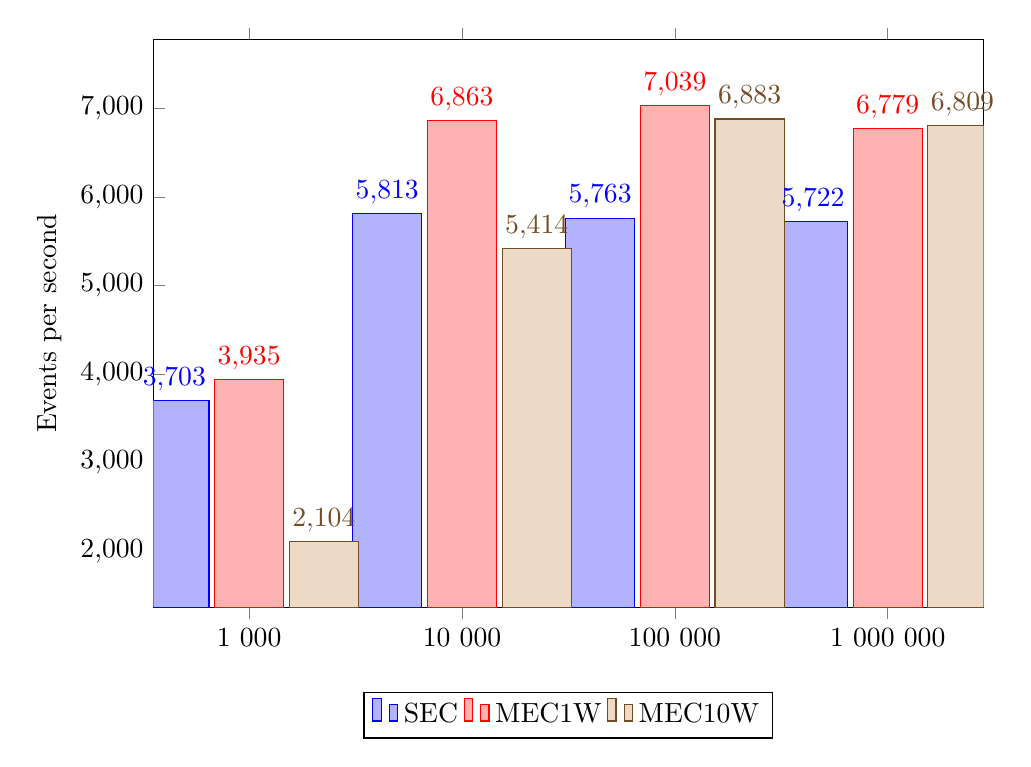
\begin{tikzpicture}
\begin{axis}[
    xtick=data,
	height=250pt,
	ylabel=Events per second,
	enlargelimits=0.15,
	legend style={at={(0.5,-0.15)},
	anchor=north,legend columns=-1},
	ybar,
	bar width=25pt,
	symbolic x coords={1 000, 10 000, 100 000, 1 000 000},
	nodes near coords,
	nodes near coords style={above}
]
\addplot coordinates {(1 000,3703) (10 000,5813) (100 000,5763) (1 000 000,5722)}; % SEC
\addplot coordinates {(1 000,3935) (10 000,6863) (100 000,7039) (1 000 000,6779)}; % MEC1W
\addplot coordinates {(1 000,2104) (10 000,5414) (100 000,6883) (1 000 000,6809)}; % MEC10W
\legend{SEC, MEC1W, MEC10W}
\end{axis}
\end{tikzpicture}
\\
These tests are run with 1 logical core on a "Intel(R) Core(TM) i7-7600U CPU @ 2.80GHz" (2 cores x 2 threads per core = max 4 logocal cores) and 24GB RAM.

\begin{itemize}
    \item Why is the MEC10W slower?
    \item Why are the runs on the 1 000 dataset generally lower?
\end{itemize}

By using all CPU cores available (4) instead of a single one, we can take better advantage of Gos concurrency model, and raise the throughput when using multiple workers and CPUs:

\pgfplotsset{scaled y ticks=false}
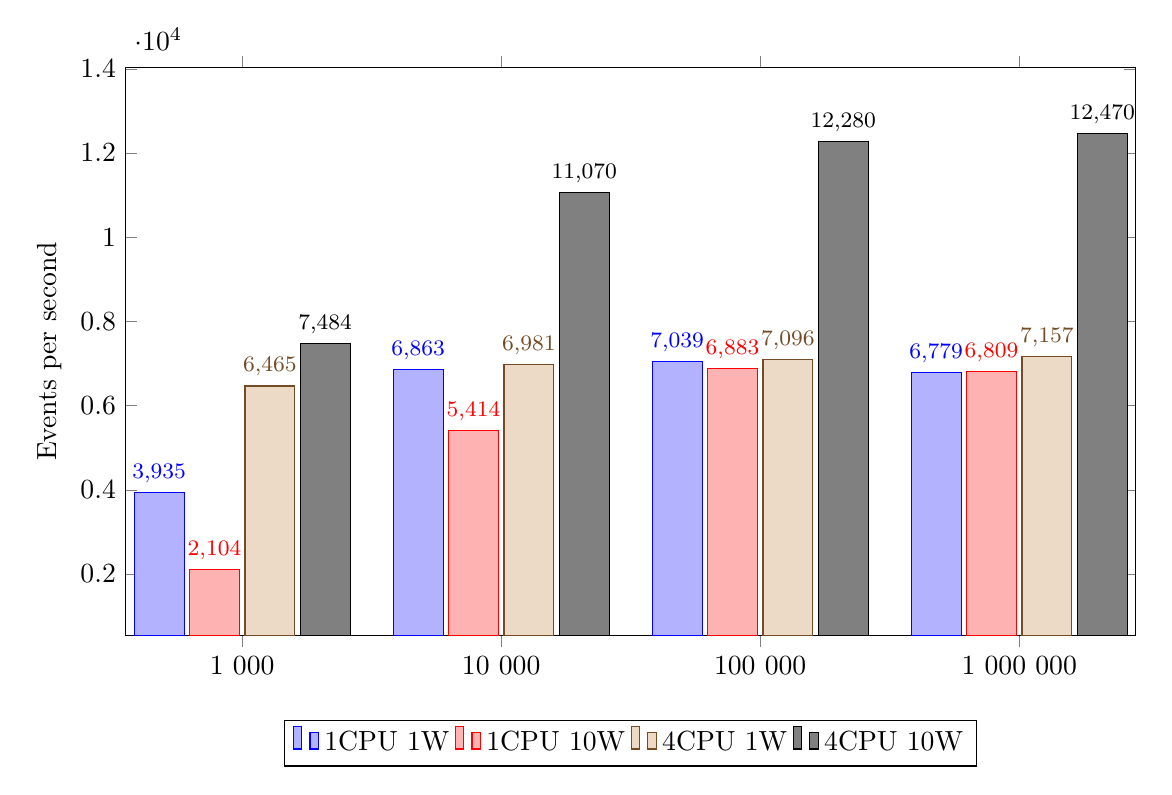
\begin{tikzpicture}
\begin{axis}[
    xtick=data,
    width=410pt,
	height=250pt,
	ylabel=Events per second,
	enlargelimits=0.15,
	legend style={at={(0.5,-0.15)},
	anchor=north,legend columns=-1},
	ybar,
	bar width=18pt,
	symbolic x coords={1 000, 10 000, 100 000, 1 000 000},
	nodes near coords,
	nodes near coords style={above, font=\footnotesize},
]
\addplot coordinates {(1 000,3935) (10 000,6863) (100 000,7039) (1 000 000,6779)}; % 1CPU 1W
\addplot coordinates {(1 000,2104) (10 000,5414) (100 000,6883) (1 000 000,6809)}; % 1CPU 10W
\addplot coordinates {(1 000,6465) (10 000,6981) (100 000,7096) (1 000 000,7157)}; % 4CPU 1W
\addplot coordinates {(1 000,7484) (10 000,11070) (100 000,12280) (1 000 000,12470)}; % 4CPU 10W
\legend{1CPU 1W , 1CPU 10W , 4CPU 1W , 4CPU 10W}
\end{axis}
\end{tikzpicture}

\begin{itemize}
\item Why is there a dip for 1CPU,10W when using a dataset of 1 000 events?
\item Why are the results of 1CPU,1W, 1CPU,10W and 10CPU,1W generally the same?
\item What can we say about 1CPU,10W "catching up" to the others around 100 000 events?
\end{itemize}

\section{Implemented a new rule format}
This format relies less on the extensive use of Regexes, as we saw in the rules used by Simple Event Correlator.

\subsection{Sigma}
\url{https://github.com/Neo23x0/sigma}

Sigma is an open standard for rules that are used to generically describe searches in log data. It is primarily used as a high-level rule that transcompile into SIEM queries like Splunk, ElasticSearch, QRadar, etc.

The rules are written in YAML (Yet Another Markup Language), and are key-value based.

\com{Testing}
\todo{Do somethiing}
\n{Testing note}
\begin{lstlisting}
title: Quick Execution of a Series of Suspicious Commands
id: 61ab5496-748e-4818-a92f-de78e20fe7f2
description: Detects multiple suspicious process in a limited timeframe
status: experimental
references:
    - https://car.mitre.org/wiki/CAR-2013-04-002
    - https://car.mitre.org/wiki/CAR-2013-04-003
author: juju4
modified: 2012/12/11
tags:
    - car.2013-04-002
logsource:
    category: process_creation
    product: windows
detection:
    selection:
        CommandLine:
            - ipconfig
            - arp
            - echo
    timeframe: 10s
    condition: selection | count() by MachineName > 3
falsepositives:
    - False positives depend on scripts and administrative tools used in the monitored environment
level: low
\end{lstlisting}

\subsection{Context}
\todo{What is context?}

\subsection{The Context Engine}
We are using a shared map between the "workers" of the application.

\subsection{Results}

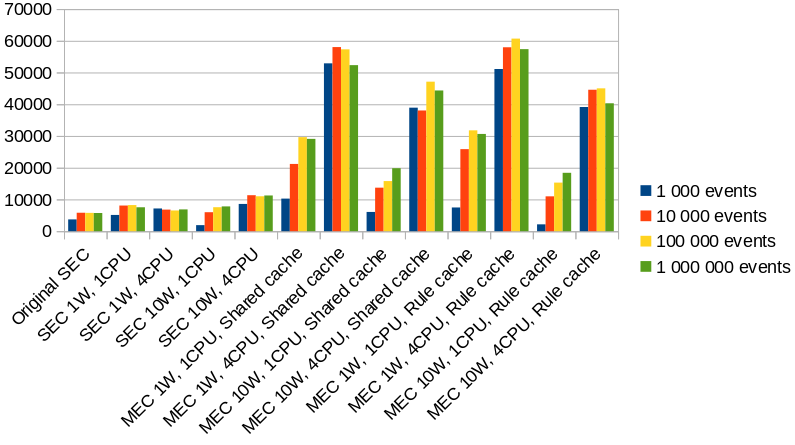
\includegraphics[scale=0.525]{figures/new-rule-format/performance.png}
\\
Min hypotese her, er at ved å bruke flere regler som trenger kontekst, så vil vi få et enda større sprang mellom shared og rule-based caching enn det vi ser over.
\\
Under har jeg generert 1000 regler og kjørt MEC på disse. Høyere søyle er bedre. Det er ganske tydelig at event-per-sekund her faller drastisk, da det må itereres over flere regler (2 vs 1000).
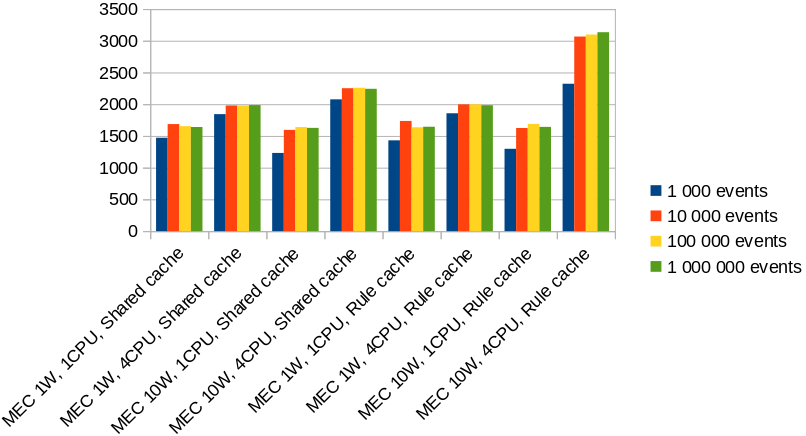
\includegraphics[scale=0.525]{figures/new-rule-format/performance-2.png}
\\
Som forventet så ser vi at rule-cache med 10W og 4CPU gir en 39.77\% økning sett opp imot 10W og 4CPU og shared caching.

Det som er interessant her er at det er liten forskjell mellom (1W, 1CPU), (10W, 1CPU) og (1W, 4CPU) mellom de forskjellige cache-typene. Dette gir mening, da lavt antall workers og CPU ikke drar ordentlig nytte av rule-based caching, og vil da falle ned til samme hastighet som shared cache.
\chapter{Introduction}
\label{chap:introduction}

\iffalse
Scrutiny of the introduction - http://sepwww.stanford.edu/sep/prof/Intro.html
\fi

\iffalse
The review

Pick out about 3-10 papers providing a background to your research and say something about each of them. You could paraphrase a sentence or two from each abstract. The review is not intended to be a historical review going back to Newton or Descartes. Try to find a few papers by your office mates, your advisor, your predecessors, or other associates. That way you might find somebody to give you helpful criticism!

Anyone can follow these instructions and write a review that looks presentable. Where intelligence and skill are required is in organizing the review so that it leads up to something, namely, to your claim.
\fi

\iffalse
The claim

The most important part of the introduction is buried in the middle. It is the claim. The claim is where you claim your work is a worthwhile extension of the review you just wrote. If someone says your writing is "unmotivated," they are not insulting your humanity; it just means they can't find your claim.

In your claim you should use the personal pronoun "I" (or "we" if you aren't the sole author). The word "I" tells people where common knowledge runs out and your ideas begin. If you are writing a doctoral dissertation or an article for a refereed journal, then you should be making a new contribution to existing knowledge. Your paper is not acceptable without an identifiable claim.
\fi

\iffalse
I believe that by using a more modern pipeline, programming language and ruleset for event correlation, we can improve not just the correlation throughput (events per second), but also make it simpler for security analysts to create, edit and manage correlation rules.
\fi

\iffalse
The agenda

An agenda is found at the end of many introductions. It summarizes what you will show the reader as your paper progresses. Your agenda will be dull if it is merely a recital of the topics you will cover. Your agenda should tell how your paper works to fulfill your claim. In this way your agenda should clarify your claim.

The agenda is not as important as the review and the claim. Keep it short.

Occasionally you will be fortunate enough to be writing about something in which some of your conclusions can be made in simple statements. If so, state them early, right after your agenda. You aren't trying to write a mystery! Many more people will begin reading your paper than will finish reading it. Motivate them to finish! Unfortunately, many technical papers do not lend themselves to early conclusions.
\fi
\iffalse
In this thesis, I will first give some background into the field of correlating event technologies, and give an overview of the state-of-the-art. Then I will explain the methods I have used to measure and analyze our results. After this, I will go into detail on our results, before we then discuss and analyse our results. Finally, I will conclude with some further work to be done.


\makebox[\linewidth]{\rule{\paperwidth}{0.4pt}}
\fi

This field is maturing, as focus has shifted from network monitoring and detection, to a more endpoint-centric approach....

\section{Problem description}
\label{sec:problemdescription}

We are seeing a movement away from network-based monitoring and detection. There are several reasons for this.

\begin{itemize}
    \item Increased usage of encrypted communications, as encryption has become standard and more popular than ever before. The continued introduction of other privacy-enhancing technologies like DNS-over-TLS/DNS-over-HTTPS will continue to hinder network-based monitoring and detection from being effective.
    \item Endpoints are no longer static inside a business network. Employees bring the computers with them outside of the office. Sometimes connected to their business' network via a Virtual Private Network (VPN), sometimes not.
    \item Network-based detection only give you a glimpse at what happens on the wire. There is not visibility into what is happening on the individual endpoints connected to the network.
\end{itemize}
The trend seems to be moving more towards host-based monitoring and detection instead. Traditionally, this has been frowned upon, as CPU-intensive agents would have to be installed on the endpoints. But now we are seeing higher performing agents, as well endpoints with more performant hardware. There are several advantages to moving to endpoint monitoring and detection.

\begin{itemize}
    \item Host-based detection and response makes it easier to detect anomalies and badness using either 3rd party software, or built-in capabilities of the OS.
    \item We are not bound to a particular network for protection, so we are still covered monitoring and detection-wise when on the move.
    \item There is a constant development to allow further insight into what is happening on the endpoint by the OS-vendors.
\end{itemize}

Current detection analysis is based on aggregating log files into a centralized system known as a System Information and Event Management (SIEM) system. Traditionally in a SIEM, logs are analyzed after-the-fact. This has several drawbacks:

\begin{itemize}
    \item Security monitoring is reactive.
    \item Requires actively hunting for bad events.
\end{itemize}

Another huge problem with pure SIEM-based logging, as companies are collecting more and more logs, actively hunting for badness in those logs are becoming harder and more complex. I single log item from a single source is not enough to properly analyze what has happened in a system. Only by cross-correlating several log lines and log sources are we able fully understand the situation at hand.

An example of this might be that we have a log item X. This means Y and is not a indication of badness in and of itself.
But if we also see log item Y right before log item X, that could be a indication of attack-pattern X. Which is a known Indicator of Compromise.



\iffalse
FROM http://folk.uio.no/josang/papers/MJ2018-ICCSP.pdf
Current threat detection analysis approaches include aggregation of log files in a centralized system known as security information and event management (SIEM) which performs inspections
and flags anomalies. A SIEM system collects logs by deploying
multiple collection agents to gather security-related events from
end-user devices, servers, intrusion detection systems (IDS), intrusion prevention systems (IPS) and firewalls, network devices such as
routers and DNS servers and more. In particular, one resource that
has received considerable attention for endpoint visibility has been
Sysmon; a Windows system service and device driver that monitors
and logs system activity of Windows workstations. Approaches for
threat detection using Sysmon have been proposed mainly focusing
on search engines (NoSQL database systems) or graph databases.
\fi

\section{Justification, motivation and benefits}
\label{sec:justificationmotivationandbenefits}
...
There are several benefits of this approach. We are using more modern, industry-standard technology which improves scalability, availability and performance.

\section{Research questions}
\label{sec:researchquestions}

\begin{itemize}
\item How can we improve event correlation/the SEC algorithm...? Hvordan kan vi forbedre event log analyse?
Implementerer en mer effektiv versjon.
    \item How can we make event log analysis and correlation faster using a compiled programming language (Go) rather than a dynamic, interpreted language like Perl.
    \item How can we make event log correlation simpler for the analyst by utilizing a common alert format for writing and sharing rules, instead of the heavily regular expression-based apporach of SEC?
    \item How can we further improve the distributed nature of log ingestion and processing by using queuing technologies and a shared in-memory cache for context-information between the event analyzers.
    \item Does correlating events reduce the number of false positives, and therefore avoid "alert fatigue"?
\end{itemize}

\section{Planned contributions}
\label{sec:plannedcontributions}

This thesis will:

\begin{itemize}
    \item Implement and detail a system for correlating Windows Event Logs in near real time. Using Go.
    \item Analyze benefits and drawbacks of using our system versus other tools.
    \item Show how the system performs on real world data, with a focus on measures to reduce the number of false positives.
    \item Contribute rules for common attack techniques back to the community, that require correlation to avoid a high false-positive rate.
\end{itemize}


\section{Thesis Outline}
\label{sec:thesisoutline}

First, we will.... % includes latex files from the same directory
\chapter{Literature review}
\label{chap:literaturereview}

\chapter{Implementation}
\label{chap:implementation}
This has the description of how you actually went about implementing the project.  This should be focused on the interesting challenges and how those related to the project.

\todo{add more here}

\begin{figure}[h]  %t top, b bottom, p page | you can also use h to try to get the figure to appear at the current location
  \centering
  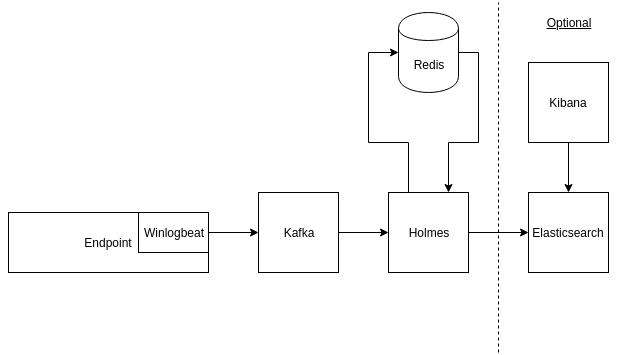
\includegraphics[width=.85\textwidth]{figures/holmes-architecture}
  \caption[An example figure.]{Minimal architecture. Every single node can be scaled both vertically and horizontally.}
  \label{fig:example}
\end{figure}
\iffalse
\include{inc/packages} % could be called Methodology or methods or any filename 
\include{inc/structure} % could be results
\chapter{Discussion}
\label{chap:discussion}

\section{Limitations of the study}
\label{sec:limitations}

\section{Future work}
\label{sec:futurework}

\todo{What could be expanded further upon in the future?}
\todo{Are there any experiments that we could have done, but didn't have the time to do? What could they tell us that we already didn't know?}
\chapter{Conclusion}
\label{chap:conclusion}
\fi
\ifthenelse{\boolean{HarvardCitations}}{%
	\bibliographystyle{agsm} % used for Harvard style references. Names - Humanities & Interaction Design
}{%
	\bibliographystyle{ntnuthesis/ntnuthesis} %used for Vancover style references. Numbers - Computer Science & Physics
}

\bibliography{MastersExample}

\appendix
\include{inc/rawdata}

\end{document}
